%% abtex2-modelo-trabalho-academico.tex, v-1.9.6 laurocesar
%% Copyright 2012-2016 by abnTeX2 group at http://www.abntex.net.br/
%%
%% This work may be distributed and/or modified under the
%% conditions of the LaTeX Project Public License, either version 1.3
%% of this license or (at your option) any later version.
%% The latest version of this license is in
%%   http://www.latex-project.org/lppl.txt
%% and version 1.3 or later is part of all distributions of LaTeX
%% version 2005/12/01 or later.
%%
%% This work has the LPPL maintenance status `maintained'.
%%
%% The Current Maintainer of this work is the abnTeX2 team, led
%% by Lauro César Araujo. Further information are available on
%% http://www.abntex.net.br/
%%
%% This work consists of the files abntex2-modelo-trabalho-academico.tex,
%% abntex2-modelo-include-comandos and abntex2-modelo-references.bib
%%

% ------------------------------------------------------------------------
% ------------------------------------------------------------------------
% abnTeX2: Modelo de Trabalho Academico (tese de doutorado, dissertacao de
% mestrado e trabalhos monograficos em geral) em conformidade com
% ABNT NBR 14724:2011: Informacao e documentacao - Trabalhos academicos -
% Apresentacao
% ------------------------------------------------------------------------
% ------------------------------------------------------------------------

\documentclass[
	% -- opções da classe memoir --
	12pt,				% tamanho da fonte
%	openright,			% capítulos começam em pág ímpar (insere página vazia caso preciso)
%	twoside,			% para impressão em recto e verso. Oposto a oneside
    oneside,			% Oposto a twoside
	a4paper,			% tamanho do papel.
	% -- opções da classe abntex2 --
	%chapter=TITLE,		% títulos de capítulos convertidos em letras maiúsculas
	%section=TITLE,		% títulos de seções convertidos em letras maiúsculas
	%subsection=TITLE,	% títulos de subseções convertidos em letras maiúsculas
	%subsubsection=TITLE,% títulos de subsubseções convertidos em letras maiúsculas
	% -- opções do pacote babel --
	english,			% idioma adicional para hifenização
	french,				% idioma adicional para hifenização
	spanish,			% idioma adicional para hifenização
	brazil				% o último idioma é o principal do documento
	]{abntex2}

% ---
% Pacotes 
% ---
\usepackage{lmodern}			% Usa a fonte Latin Modern			
\usepackage[T1]{fontenc}		% Selecao de codigos de fonte.
\usepackage[utf8]{inputenc}		% Codificacao do documento (conversão automática dos acentos)
\usepackage{lastpage}			% Usado pela Ficha catalográfica
\usepackage{indentfirst}		% Indenta o primeiro parágrafo de cada seção.
\usepackage{color}				% Controle das cores
\usepackage{graphicx}			% Inclusão de gráficos
\usepackage{microtype} 			% para melhorias de justificação
\usepackage{filecontents}       % Used so that the external files can be placed in this file

\usepackage[brazilian,hyperpageref]{backref}	 % Paginas com as citações na bibl
\usepackage[alf]{abntex2cite}	% Citações padrão ABNT

% ---
% CONFIGURAÇÕES DE PACOTES
% ---

% ---
% Configurações do pacote backref
% Usado sem a opção hyperpageref de backref
\renewcommand{\backrefpagesname}{Citado na(s) página(s):~}
% Texto padrão antes do número das páginas
\renewcommand{\backref}{}
% Define os textos da citação
\renewcommand*{\backrefalt}[4]{
	\ifcase #1 %
		Nenhuma citação no texto.%
	\or
		Citado na página #2.%
	\else
		Citado #1 vezes nas páginas #2.%
	\fi}%
% ---
\newcommand{\basePath}{/var/www/html/meninadasbalas/project/monografia/latex}

% ---
% Informações de dados para CAPA e FOLHA DE ROSTO
% ---
\titulo{Site e-commerce para empresa do ramo alimentício}
\autor{Renan Marcel Ferreira Dias}
\local{Brasil}
\data{Junho de 2017}
\orientador{André Bernardi}
\instituicao{%
  Universidade Federal de Itajubá -- UNIFEI
  \par
  Instituto de Engenharia de Sistemas e Tecnologia da Informação
  \par
  Engenharia da Computação}
\tipotrabalho{Trabalho Final de Graduação}
% O preambulo deve conter o tipo do trabalho, o objetivo,
% o nome da instituição e a área de concentração
\preambulo{Monografia referente ao Trabalho Final de Graduação do curso de Engenharia da Computação da Universidade Federal de Itajubá}
% ---



% ---
% Configurações de aparência do PDF final

% alterando o aspecto da cor azul
\definecolor{blue}{RGB}{41,5,195}

% informações do PDF
\makeatletter
\hypersetup{
     	%pagebackref=true,
		pdftitle={\@title},
		pdfauthor={\@author},
    	pdfsubject={\imprimirpreambulo},
	    pdfcreator={LaTeX with abnTeX2},
		pdfkeywords={abnt}{latex}{abntex}{abntex2}{trabalho acadêmico},
		colorlinks=true,       		% false: boxed links; true: colored links
    	linkcolor=blue,          	% color of internal links
    	citecolor=blue,        		% color of links to bibliography
    	filecolor=magenta,      		% color of file links
		urlcolor=blue,
		bookmarksdepth=4
}
\makeatother
% ---

% ---
% Espaçamentos entre linhas e parágrafos
% ---

% O tamanho do parágrafo é dado por:
\setlength{\parindent}{1.3cm}

% Controle do espaçamento entre um parágrafo e outro:
\setlength{\parskip}{0.2cm}  % tente também \onelineskip

% ---
% compila o indice
% ---
\makeindex
% ---

% ----
% Início do documento
% ----
\begin{document}

% Seleciona o idioma do documento (conforme pacotes do babel)
%\selectlanguage{english}
\selectlanguage{brazil}

% Retira espaço extra obsoleto entre as frases.
\frenchspacing

% ----------------------------------------------------------
% ELEMENTOS PRÉ-TEXTUAIS
% ----------------------------------------------------------
% CAPA ---------------------------------------------------------------------- %
\imprimircapa

% FOLHA DE ROSTO ------------------------------------------------------------ %
\imprimirfolhaderosto*

% DEDICATORIA --------------------------------------------------------------- %
\begin{dedicatoria}
  %% Dedicatória

\vspace*{\fill}
\centering
\noindent
Dedico este tabalho ao meu bebê que está por vir. Sendo Alice ou Samuel, é e será a o bebê, a criança, a pessoa mais amada deste mundo.
\vspace*{\fill}

  % Dedicatória

\vspace*{\fill}
\centering
\noindent
Dedico este tabalho ao meu bebê que está por vir. Sendo Alice ou Samuel, é e será a o bebê, a criança, a pessoa mais amada deste mundo.
\vspace*{\fill}

\end{dedicatoria}

% AGRADECIMENTOS ------------------------------------------------------------ %
\begin{agradecimentos}
  % Agradecimentos

Agradeço a todos os amigos envolvidos em todo o processo deste trabalho e também a todos os desenvolvedores da comunidade Drupal, que trabalham termos um software livre de qualidade. Agradeço também aos meus pais, que sempre me incentivaram a seguir um objetivo com determinação e ajudaram em todas as conquistas. Agradeço especialmente a minha esposa Renata, que me ajudou pacientemente, corrigindo, dando idéias e mantendo meu foco nos objetivos, não só deste projeto, mas de todos os outros, passados, presentes e tenho certeza que nos futuros também.

\end{agradecimentos}

% EPIGAFE ------------------------------------------------------------------- %
\begin{epigrafe}
  % Epigrafe

\vspace*{\fill}
\begin{flushright}
    \textit{``Não vos amoldeis às estruturas deste mundo, \\
    mas transformai-vos pela renovação da mente, \\
    a fim de distinguir qual é a vontade de Deus: \\
    o que é bom, o que Lhe é agradável, o que é perfeito.\\
    (Bíblia Sagrada, Romanos 12, 2)}
\end{flushright}

\end{epigrafe}

% RESUMO -------------------------------------------------------------------- %
\setlength{\absparsep}{18pt} % ajusta o espaçamento dos parágrafos do resumo
\begin{resumo}
  % Resumo

Este é um projeto de um sistema web de e-commerce, construido para uma empresa real do ramo alimentício com base na cidade de Itajubá em Minas Gerais. O objetivo é criar um site rápido e seguro, que entregue ao usuário uma experiência única e apresente de forma clara e informativa o produto da empresa. Alguns conteúdos serão criados para enriquecer o site e chamar a atenção do cliente para o produto.

Utilizaremos o framework e gerenciador de conteúdos Drupal construido na linguagem PHP, escolhido por sua solidez e grande comunidade de desenvolvedores. Sua versão mais recente, o Drupal 8, é uma plataforma flexivel e inovadora, com sistemas de cache bem robustos e várias API's que fornecem métodos seguros de construir um website.

Nossos objetivos poderão ser atingidos com a ajuda de módulos da comunidade Drupal e as mais novas tecnologias e tecnicas de sistemas web que forem cabíveis. O fluxo de desenvolvimento será o mais seguro para a solidez do código, utilizando o software Vagrant para garantir ambiêntes constantes e git para controle de versão. O automatizador de tarefas Gulp e os gerenciadores de pacotes NPM e Composer serão algumas das ferramentas utilizadas para facilitar os processos de instalação e programação.

Esperamos que site tenha um desempenho acima da média e testes são feitos constantemente para garantir este quesito. A mais utilizada será o GTMetrix, ferramenta de teste de performance mais completa atualmente, que ainda dá dicas de pontos para  se melhorar.

\textbf{Palavras-chave}: e-commerce. drupal. web. php. performance. seo. twig. less.

\end{resumo}

% RESUMO EM INGLES ---------------------------------------------------------- %
\begin{resumo}[Abstract]
  % Resumo em ingles

\begin{otherlanguage*}{english}
   This is the english abstract.

   \vspace{\onelineskip}

   \noindent
   \textbf{Keywords}: latex. abntex. text editoration.
\end{otherlanguage*}

\end{resumo}

% ---
% inserir lista de ilustrações
% ---
\pdfbookmark[0]{\listfigurename}{lof}
\listoffigures*
\clearpage
% ---

% ---
% inserir lista de tabelas
% ---
\pdfbookmark[0]{\listtablename}{lot}
\listoftables*
\clearpage
% ---

% ---
% inserir lista de abreviaturas e siglas
% ---
\begin{siglas}
  \item[ABNT] Associação Brasileira de Normas Técnicas
  \item[abnTeX] ABsurdas Normas para TeX
\end{siglas}
% ---

% ---
% inserir o sumario
% ---
\pdfbookmark[0]{\contentsname}{toc}
\tableofcontents*
\clearpage
% ---

% ----------------------------------------------------------
% ELEMENTOS TEXTUAIS
% ----------------------------------------------------------
\textual

\chapter{Introdução}

% =========================================================================== %
\section{O Comércio Convencional}

Quando falava-se em comércio à 20 anos atrás, pensavamos em uma estabelecimento comercial, que podiamos nos deslocar até ele, entrar e sermos atendidos por um vendedor. Um lugar onde podiamos ver o produto que queriamos comprar, tocar, analisar sua cor e sentir seu cheiro. Após escolher, pagariamos com dinheiro ou cheque e levariamos para a casa o produto.


% =========================================================================== %
\section{A Internet}

O comércio muda muito sua cara de tempos em tempos, mas nunca tivemos um salto tão grande na forma de comprar e vender mercadorias como nos últimos 20 anos. Desde 1995 quando a Amazon, gigante americana do comércio eletrônico, fez sua primeira venda online, em uma época que o Brasil ainda estava conhecendo a internet, muita coisa mudou. Novas tecnologias nos permitem comprar e vender sem sair do conforto de nossas casas e também à pagar, receber e movimentar dinheiro por dispositívos móveis que estão conectados a internet 24h por dia, sem ter que ir ao banco e enfrentar filas.

Todas estas mudanças fizeram com que as empresas que quisesem continuar no mercado e ter sucesso nos tempos atuais, mudassem sua maneira de fazer negócio. A importância do comércio físico, apesar de grande, está em decadência, e a presença na web é um requisito fundamental. Empresas que são recordistas em vendas em lojas físicas, como por exemplo a Casa Bahia e o Magazine Luiza, investiram e ainda estão investindo pequenas fortunas na criação e manutenção de seus websites e aplicativos móveis.


% =========================================================================== %
\section{E-commerce}

Comércio eletrônico, e-business ou e-commerce são termos usados para definir qualquer tipo de negociação que envolva trasmissão de dados pela internet\cite{WhatIsEcommerce}. Vários tipos de negócios se encacham nesta definição, de sites de venda de camisetas à sistemas online de bancos onde o cliente pode fazer transações e contratar serviços online.

\subsection{Vantagens}

Uma loja online permite a uma empresa vender produtos com um preço diferenciado, beneficiando os compradores. Isso acontece pois seus gastos são menores, principalmente com vendedores e espaços físicos.

No modo tradicional de comércio, uma empresa que queira ter grande visibilidade, tem que desembolsar grandes quantidades de capital para se intalar em lugares estratégicos, onde o fluxo de compradores é grande. Na internet, um site e-commerce de uma empresa pequena tem tantas chances quanto o de uma empresa com maior capacidade financeira. Tudo depende da qualidade e segurança do site e da força do marketing. Com muito pouco capital, faz-se campanhas de marketing online que atingem muito mais pessoas por dia que uma loja física no melhor ponto de comércio do mundo, seja ele onde for. Isso acontece pois na internet não há barreiras geográficas, pode-se comprar e vender para qualquer lugar do mundo.

\begin{itemize}
  \item Facilidade e conforto de fazer compras sem sair de onde está.
  \item Maior disponibilidade de lojas e produtos.
  \item Melhores condições para pesquisa e comparação de preços.
  \item Sem filas ou espera por vendedores ou atendentes livres.
  \item Acesso a produtos de várias regiões do país e do mundo.
  \item Fácil acesso a promoções e cupons de desconto.
  \item Lojas abertas o tempo todo.
  \item 
\end{itemize}

\subsection{Desvantagens}

Nem tudo é perfeito no mundo do e-commerce. Salvo excessões, estas são algumas desvantagens deste tipo de negócio.

\begin{itemize}
  \item Está sujeito a falhas e pode ser vulnerável a ataques.
  \item Em transações com cartões de crédito, há o risco de roubo ou fraudes.
  \item Impossibilita a inspeção física do bem a ser adquirido.
  \item Preço e tempo de entrega podem inviabilizar o negócio.
  \item Dificuldade e demora no retorno ou troca de mercadorias
  \item Nem tudo pode ser vendido online, como por exemplo comidas perecíveis.
  \item Produtos de alto custo como jóias não tem segurança suficiente para serem despachados como encomenda.
  \item Não há o toque pessoal, interação entre cliente e comprador, que pode fazer diferença na concretização de uma venda.
\end{itemize}


% =========================================================================== %
\section{Ambiente de Desenvolvimento}

Existem várias maneiras de se criar um website, com várias linguagens e frameworks disponíveis. Linguagens como PHP, Ruby, Java e C# estão entre as linguagens mais utilizadas \cite{UsageStatistics}. Fazer um website simples do zero não é tarefa difícil. Porém no caso de um e-commerce, onde segurança e usabilidade são fatores chave para o sucesso do negócio, desenvolver em cima de camadas de software que já te proporciona muitas funcionalidades que serão essenciais, segurança contra ataques e falhas, além de uma comunidade de desenvolvedores que disponibiliza código e ajuda, faz desta a melhor opção. Mais adiante (!!!!!!!!colocar o capítulo!!!!!!!!), falaremos da escolha deste framework, quais eram as opções e o critério usado para a seleção.

Outra parte importante do desenvolvimento de um website é a escolha de um serviço de hosting. Servidores existem em várias partes do mundo e para sites de pequeno tráfego podemos encontrar por preços que vão de 100 reais por ano por um servidor compartilhado a 500 reais por ano uma maquina virtual exclusiva. A qualidade do servidor, sua conexão com a internet e localização física podem fazer muita diferença.

Como mais um fator a se considerar, temos o domínio. Domínio é o endereço que o usuário vai usar no browser para utilizar o website. Alguns domínios podem ser contratados em websites especializados de graça, como por exemplo o domínio `.tk` no `site www.dot.tk`. Estes domínios tem pouca visibilidade nos motores de busca e tem pouca confiança dos usuários por não serem amplamente utilizados. No Brasil, os domínios com melhor visibilidade e confiança são o `.com.br` e o `.com`, que por um custo não muito elevado, por volta de 50 reais, podem ser contratados por um ano.

É muito importante para o desenvolvedor de websites, garantir que o código que foi feito, funcione no servidor da mesma maneira que funcionou no ambiênte de desenvolvimento, computador pessoal ou notebook, de todos que participaram do projeto. Para não termos que instalar o mesmo sistema operacional e softwares em todos os computadores que forem utilizados, o uso de uma maquina virtual é a saida. Em uma maquina virtual, com as mesmas configurações do servidor que será utilizado e de fácil replicação nas máquinas de desenvolvimento, este problema é solucionado.

Outra parte esencial para o desenvolvimento de qualquer tipo software, principamente em web, são os softwares gerenciadores de pacotes e automatizadores de tarefas. Gerenciadores de pacotes ajudam na controle das bibliotecas que serão utilizadas e suas versões. Algumas delas já tomam conta de possíveis dependências que estas podem ter e também facilitam o upgrade ou downgrade quando necessários. Automatizadores de tarefas são úteis principalmente no front-end de uma aplicação web. Muitas tarefas como compilação, minificação e manipulação de arquivos podem ser feitas de forma automática, economizando tempo de desenvolvimento e ajudando o programador a focar no código.

% =========================================================================== %
\section{Tecnologias de Web}

Em aplicações web, temos código que executam tanto no servidor, quanto no cliente. O servidor é onde todas as informações estão guardadas em um banco de dados e o código que é executado nesta fase é chamado de back-end. Já no cliente, normalmente um browser, o código é geralmente para melhorar a experiência do usuário, mostrar as informações de forma mais clara, carregar informações dinamicamente sem mudar de página, fazer interações com o usuário e utilizar efeitos em elementos da página. Esta parte é chamada de front-end.


% =========================================================================== %
\section{SEO, Performance e Segurança}

\subsection{Search Engine Optimization}

Otimização para motores de busca (do inglês) são um conjunto de técnicas utilizadas em websites para melhorar o seu posicionamento em buscadores como o Google, Bing e Yahoo. Esta é uma parte essencial para a empresa que quer ter visibilidade na internet. Quanto mais próximo do topo em motores de busca, maior a chance de usuários clicarem no seu link e visitarem seu website. Hoje em dia existem empresas e proficionais especializados em SEO, dada a importância do assunto.

\subsection{Performance}

O tempo de carregamento e de renderização de um website impactam muito na quantidade de usuários que ele vai reter. Segundo Shaun Anderson \cite{LoadTime}, SEO da empresa MBSA Marketing LTD, cada segundo a mais que um website demora para carregar, a taxa de abandono aumenta cerca de 6\%, chegando a 25\% após 4 segundos. Além da perda de potenciais clientes, sites com performance probre tem seu rankeamento prejudicado em motores de busca. Existem várias ferramentas e softwares que testam a velocidade e dão dicas para melhora-la, como por exemplo o PageSpeed Insights do Google e o YSlow do Yahoo.

\subsection{Segurança}

Quando trabalhamos com cartões de crédito e informações confidenciais de clientes, temos que preocupar com a segurança destes dados. São quatro os principais fatores a se levar em consideração \cite{SecurityEcommerce}:

\begin{itemize}
  \item Privacidade: Todas as informações (!!!!!!!!!!!!!!!!!!)sensitivas dos clientes devem ser mantidas em bancos de dados seguros e longe do acesso de pessoas e empresas não autorizadas.
  \item Integridade: As informações dos clientes não devem ser modificadas ou adulteradas.
  \item Autenticação: Tanto o website quanto o cliente devem provar suas identidades um ao outro.
  \item Confirmação: É esperado que as informações trocadas sejam verificadas, para ter certeza que foram transmitidas e de forma correta.
\end{itemize}

% =========================================================================== %
\section{O Cliente}

A empresa Menina das Balas de Coco foi fundada 2010 na cidade de Itajubá, Minas Gerais. Seu produto principal e único é a bala de coco, doce típico brasileiro que costuma ser servido em festas de aniversário. O nome da empresa vem de como era conhecida a fundadora na faculdade, onde cursava Letras e vendia suas primeiras balas. A partir dai, foi-se aperfeiçoando as tecnicas de fabricação e melhorando o produto. Hoje a empresa tem mais de 20 sabores de balas que podem ter recheios diversos sabores, além da bala gelada e a original bala bombom, com cobertura de chocolate. Sua principal forma de vendas é por perfis em redes sociais.


\chapter{Objetivo}

% =========================================================================== %
\section{Objetivo Geral}

O objetivo deste trabalho é criar um website e-commerce para a empresa Menina das Balas de Coco. O site terá uma area de publicação de notícias, tipo blog e também cadastro de produtos do tipo bala de coco. Deverá ser possível passar por todo o fluxo de compras no site, sendo aceitável um redirecionamento na hora do pagamento, para plataforma especializada. A performace do website deverá ser medida em softwares adequados e o resultado deve ser acima da média. Os dados dos clientes devem ser captados e mantidos de forma segura. Este website deve servir também como um portal de informações sobre a empresa com boa indexação nos mecanismos de busca, para melhor visibilidade na web. O custo de instalação e manutenção devem ser mínimos.

% =========================================================================== %
\section{Objetivo Específico}

\subsection{E-commerce}

Como todo e-commerce, o site deverá ser capaz de guiar o usuário no processo de compra do produto a ser vendido. A facilidade de uso deste mecanismo é fundamental para o sucesso do negócio. Deverá ser possível para o administrador do site cadastrar o produto e todas as suas variantes de sabor, recheio e cobertura, com o preço em Reais (BRL), um texto de apresentação do produto e imagens. Vitrines destes produtos deverão estar em todas as páginas do site, principalmente na homepage. Por ser a principal razão do site, os produtos deverão ter destaque sempre que mostrados, com uma cor que contraste com o tema do site.

% =========================================================================== %
\subsection{Funcionalidades}

\subsubsection{Notícias}
O site deverá possuir um método de postagem de notícias, informações sobre produtos ou a empresa, como um blog.
Este conteúdo terá um título, uma imagem e um corpo que possa conter texto, imagens e videos. Na pagina de descrição deste post, deverá ser possível compartilha-los em redes sociais, como Facebook e Twitter com simples botão. Na página inicial do site, deverá haver uma breve listagem dos posts mais recentes, somente o título e a imagem com link para uma página com o conteúdo completo.

\subsubsection{Baner}
Teremos também um baner na homepage, utilizado em estrutura carrosel. Este baner será uma imagem da largura da tela, com um título e um texto complementar curto sobrepondo esta imagem. O objetivo deste é dar destaque a qualquer tipo de promoção, postagem ou produto do site.

\subsubsection{Usuários}
A aplicação deverá permitir o cadastro de usuários, tanto para identificação na hora da compra, como para a postagem opiniôes e ingresso em lista de e-mail. Será dado como alternativa ao formulário de cadastro o registro por redes sociais, facilitando o processo. O usuário deverá prover pelo menos nome, email e estado para finalizar o cadastro. Ao iniciar o processo de checkout de uma compra, será requisitado informações adicionais que sejam necessárias, como endereço e documentos.

\subsubsection{Review}
Para dar espaço a opiniões sobre o produto para os clientes, teremos a possibilidade de ter link enviado por e-mail para opiniões sobre os produtos que forem comprados. Este e-mail será enviado pelo site e o conteúdo publicado somente com o aval do administrador. Estes conteúdos terão uma vitrine na homepage e serão mostrados nas páginas dos respectivos produtos.

\subsubsection{Opinião}
Além de opinar sobre o produto, o cliente poderá ser requisitado a dar sua opinião sobre a empresa. Esta informação poderá ser utilizada na homepage, filtrada pelo administrador.

\subsubsection{Páginas de FAQ e Contato}
Para facilitar para os clientes e potencialmente diminuir a necessidade de atendimento direto, o site deverá ter uma página com as perguntas mais frequêntes e suas respostas. Este conteúdo deverá ter fácil sistema de cadastro para o administrador e links em lugares de fácil acesso.

% =========================================================================== %
\subsection{Performance e SEO}

Utilizaremos o máximo possível de técnicas para melhorar a performance do site. Ao final, apresentaremos os testes de performance, comparando-o com os sites mais acessados da internet no momento. É esperado que o tempo de carregamento médio do site fique abaixo dos 3 segundos para proporcionar a melhor experiência para o usuário.

Com uma performance boa, teremos o primeiro passo dado para um boa indexação do site nos mecanismos de busca. Utilizaremos e aprenderamos sobre tecnicas como metatags, microdata, estrutura do HTML e midias sociais.

\subsection{Tecnologias}

Como objetivo final, iremos pesquisar e aprender sobre as tecnologias mais utilizadas para desenvolvimento web, o que nos ajudará a atingir todos os outros objetivos citados acima da melhor maneira possível.

\chapter{Método}

Neste capítulo descreverei as tecnologias utilizadas e o por que de sua escolha.

% =========================================================================== %
\section{Pré-desenvolvimento}

\subsection{Hosting}
Como dito anteriormente, temos muitas opções de servidores para instalarmos este e-commerce. Para a escolha, foi levada em consideração a recomendação dos usuários do framework que será utilizado (será explanado na próxima seção) postado em \url{www.drupal.org/hosting}, o preço oferecido, a quantidade de domínios possíveis e o espaço em disco disponibilizado. As melhores opções na época de contatação do serviço eram:

\begin{table}
  \centering
  \begin{tabular}{ | l | l | l | l |}[Hosting]
    \hline
    Nome      & Espaço    & Domínios  & Valor         \hline
    Bluehost  & Ilimitado & 3         & R\$ 15,90/mês \hline
    Hostgator & Ilimitado & Ilimitado & R\$ 9,99/mês  \hline
    GoDaddy   & Ilimidado & Ilimitado & R\$ 10,99/mês \hline
    SiteGroud & 20 GB     & Ilimitado & R\$ 14,99/mês \hline
  \end{tabular}
  \caption{Opções de hosting para o e-commerce.}
  \label{Hosting}
\end{table}

Deste, foi escolhido o serviço da empresa Hostgator, por oferecer espaço e domínios ilimitados e o menor preço.

\subsection{Domínio}
Como também é um fator importante para SEO, foi sugerido ao cliente escolher um nome de domínio simples, facil de ser associado com a marca e com um top level domain (TLD ou domínio de nível superior) que dê credibilidade ao site como por exemplo o `.com` ou `.com.br`. No caso deste último, a indexação será melhor em uma busca nacional \cite{TLD}. Foi então combinado de usar o nome da empresa com o TLD mais utilizado, com mais de 90\% dos sites brasileiros \cite{RegistroBr}, ficando como a seguir:

\begin{figure}
  \centering
    \large
    meninadasbalas.com.br
\end{figure}

Comprado online na empresa GoDaddy \url{br.godaddy.com}, foi pago R\$ 44,99 por 1 ano de direito de uso deste domínio.

% =========================================================================== %
\section{Drupal}

Como base para o o e-commerce utilizaremos o framework e gerenciador de conteúdo Drupal.  Este software foi criado em 2000 pelo estudante universitário belga Dries Buytaert para ser um pequeno gerenciador de postagem um blog. Mais tarde em 2001, o código deste sistema foi aberto ao público, com o intuito de permitir as pessoas pudessem realizar experimentos e construir extenções. Desde então, o número de usuários vem crescendo a cada ano e sua comunidade de desenvolvedores melhorando o código diarimente. Hoje o Drupal conta com mais de 37 mil extenções \cite{DrupalModules}, chamadas de módulos, com diversas funcionalidades e utilizando as mais novas tecnologias, além de mais de 2 mil temas \cite{DrupalTheme}.

Os motivos desta escolha são:

\begin{itemize}
  \item Segurança: Muitas camadas de proteção são oferecidas pelo Drupal, desde controle de acesso de usuários à API's que protegem o sistema de ataques.
  \item Flexibilidade: Podemos usa-lo para todo e qualquer tipo de site ou serviço online e seu sistema pode ser adaptado para qualquer projeto.
  \item Comunidade: A quantidade e qualidade das extenções providas pela comunidade para adicionar as mais diversas funcionalidades.
  \item Experiencia: Prévia experiência com o framework, o que facilita o design e desenvolvimento do sistema e-commerce.
\end{itemize}

\subsection{Drupal 8}

A versão estável mais recente do Drupal é a número 8 e será a utilizada no projeto. Comparada com a versão anterior, temos um sistema de cache muito mais potênte, módulos importantes adicionados ao núcleo, a mudança do sistema de templates de PHP para Twig, segurança reforçada e novas tecnologias e padrões sendo absorvidos. 

\subsection{Núcleo}

Ao instalar o Drupal nos deparamos com um site cru, mas com várias funciolidades já prontas para serem utilizadas. Algumas delas serão de suma importância para atingirmos nossos objetivos e serão listadas abaixo, pelo nome do módulo no núcleo.

\subsubsection{Node}
O gerênciamento de conteúdo é algo nativo do Drupal, então planejaremos quais os tipos que teremos no site. Cada conteúdo, conhecido como node, pode ter campos configuráveis, que podem representar propriedades do mesmo como por exemplo título, descrição, imagem, relação com outro conteúdo, autor, entre outros. Alguns deles como titulo, autor e status de publicação são padrões para todos.

Planejamos quatro tipos de conteúdo:
\begin{itemize}
  \item Banner - Representando o baner da página inicial, tendo campos para título, um subtítulo e uma imagem.
  \item Review - Representando as opiniôes dos usuários sobre os produtos com um campo de texto e o título automático, para facilitar a criação deste conteúdo.
  \item Article - Postagens gerais de conteúdo aberto, com título, imagens e textos.
  \item Opinion - Representando os opiniôes dos usuários sobre a empresa.
\end{itemize}

Poderiamos considerar o produto também um conteúdo, mas como veremos adiante, este é uma entidade a parte, criada por um módulo da comunidade.

\subsubsection{Taxonomy}
Já pensando nos produtos, criaremos um vocabulário de taxonomia, que é uma lista de keywords utilizadas para organizar o conteúdo do site. Estas keywords serão os sabores de balas que a empresa fabrica e serão atrelados a cada produto, para facilitar a posterior filtragem e exibição destes.

\subsubsection{Views}
Modo mais comum de exibir grupos de conteúdo no Drupal, o módulo Views é um dos que na versão anterior não eram parte core e por sua importancia foi incorporado. Ele permite filtragem e ordenação por valores de propriedades e a exibição de um número específico de conteúdos. 

Com ele, faremos os blocos de baners, reviews, notícias, produtos e opiniões da homepage.
\begin{itemize}
  \item Baner: Os 3 conteúdos do tipo baner em formato de carrosel automático.
  \item Notícias: As 3 notícias mais recentes postadas.
  \item Reviews: Os 4 reviews mais visualizados.
  \item Opiniões: 3 opiniões escolhidas pelo administrador.
\end{itemize}

Além dos blocos, faremos também as páginas de listagem de produtos, reviews, opiniões e notícias.

\subsubsection{User}
Responsável pelo gerenciamento dos usuários do site e suas permissões, este módulo nos permitirá ter usuários logados com todas as informações necessárioas para o fluxo de compras e criação de conteúdo.

\subsubsection{Menu}
Este módulo, como o nome já diz, cria menus com ancoras para outros lugares do site ou sites externos. Segue a listagem dos menus do site, com nome, localização e função:

\begin{itemize}
  \item Topbar Contact Menu: Localizado no topo da página, terá apenas dois links para a página de contato.
  \item Topbar User Menu: Também no top da página, terá links de login e registro para usuários anônimos e links para detalhes da conta e sair para usuários logados.
  \item Main Menu: Menu principal, na parte superior do site com links para as páginas mais importantes.
  \item Footer Menu: No rodapé do site, menu com links para loja, página de contato e informações em geral.
\end{itemize}


% =========================================================================== %
\section{Ambiente de Desenvolvimento}

Com o framework escolhido, vamos construir o ambiênte de desenvolvimento. 

\subsection{Sistemas Operacinais e Maquina Virtual} 
Utilizarei o sistema operacional Ubuntu 16.04 e esporadicamente OSX El Capitan para desenvolvimento local e no servidor temos um CentOS 6. Para evitar problemas de compatibilidade como dito no capítulo de introdução, utilisaremos para desenvolvimento local uma maquina virtual (VM) com as mesmas configurações do servidor. O gerenciamento e configuração desta será feita por um software especializado chamado Vagrant.

Será usada uma configuração pré-definida criada por Jeff Geerling \url{www.drupalvm.com/}, Arquiteto Drupal, especificamente para o Drupal, onde o Vagrant cria uma maquina virtual e a configura especificamente para Drupal, com todos os programas e ferramentas que serão necessárias para o desenvolvimento. Alteramos somentes os pontos onde temos que imitar o servidor Hostgator, que é a versão dos softwares Apache2 e MySQL e a versão da linguagem PHP. Isso já nos garante o funcionamento estável e previsivel do nosso site em todos os ambiêntes que ele estiver instalado.

\subsection{Apache, PHP e MySQL}
Apesar do Drupal funcionar com vários softwares de servidores web, como Nginx e Hiawatha, o mais utilizado é o Apache2. Além disso, nosso servidor também roda Apache2 2.2.25, então este é a escolha inevitável. 

Para a linguagem de servidor, o Drupal 8 requer PHP na versão mínima 5.5.9 e no servidor podemos escolher entre 5.5, 5.6 e 7.0. Foi escolhido a versão 7.0 por ser mais rápida \cite{PHP7Velocidade} e possuir funcionalidades mais avançadas e seguras que a versão 5.6 \cite{PHP7}.

O software de banco de dados será o MySQL versão 5.6.32, que é a única opção no servidor e foi verificada a versão utilizada.

\subsection{Fluxo}
O código será versionado pelo software Git e salvo em repositório publico remoto mantido pela empresa Github \url{www.github.com}. Quando cada pequena tarefa for terminada, um commit é feito com uma breve descrição do que foi feito. Versões de teste serão carregadas para o servidor via SSH (\TODO), também utilizando o Git. Um subdomínio será criado para esta versão de teste, adicionando `dev.` no endereço do site. Esta versão será exclusivamente para testes e deverá ter acesso restrito ao publico em geral. Assim que uma versão estável for atingida, mesmo que sem todos os requisitos do site alcançados, esta será carregada para o ambiente de produção, no domínio principal. O objetivo deste fluxo é ter o máximo de funcionalidades possíves antes de inaugurar o site.

\subsection{Composer}
Iremos utilizar o software gerenciador de pacotes Composer para instalar o Drupal e suas dependências e posteriormente os módulos da comunidade que serão necessários. Uma boa base para o projeto pode ser o Drupal-Composer Project \url{www.github.com/drupal-composer/drupal-project}, código de configuração e scripts do Composer que montam o Drupal com a estrutura de arquivos requirida por ele.

Porém, um problema foi detectado no uso deste pacote. O Drupal é instalado em um sub-diretório do projeto e não na raiz. Isso nos impede de utilizar o domínio principal quando o site for instalado no servidor, pois os arquivos tem que estar na raiz do diretório. Para resolver isto, criei uma fork \TODO \url{https://github.com/renanmfd/drupal-project} deste projeto no Github e modifiquei todos os códigos e configurações para instalar o Drupal no diretório raíz. Esta \TODO fork foi carregada no site Packagist \url{https://packagist.org} para ficar disponível para download via Composer \url{https://packagist.org/packages/renanmfd/drupal-project}.

\TODO comando \$ composer create-project drupal-composer/drupal-project:8.x-dev meninadasbalas --stability dev --no-interaction

Com o problema sanado, podemos dar inicio ao processo de instalação do Drupal e logo após a fase de codificação do projeto.

% =========================================================================== %
\section{Front-end}

\subsection{Bootstrap}
Para o estilo ou tema do site, utilizaremos um dos melhores e mais utilizados frameworks de CSS e Javascript \cite{Bootstrap} que existe atualmente, o Boostrap. A escolha deste se deu simplesmente pelo conhecimento prévio e facilidade de uso. Com ferramentas para design responsivo e bibliotecas Javascript para funcionalidades que serão necessárias como por exemplo o carrosel de baners, este framework é a melhor opção para este projeto. No momento do desenvolvimento deste projeto a versão mais estável é a 3.

\subsection{Temas Drupal}
Na comunidade de Drupal, temos um tema Boostrap, que é uma base para sites que pretendem utilizar esta ferramenta para constriur seus layouts. Este é nosso primeiro requerimento do projeto, instalado via Composer.

\TODO comando \$ composer require drupal/bootstrap

Criaremos um sub-tema, com base no Bootstrap para Drupal que será chamado `MBC Theme`. Neste tema teremos os arquivos de CSS, imagens utilizadas pelo CSS, Javascript, templates Twig e um arquivo de PHP onde podemos modificar e adicionar as variáveis que são passadas os templates. 

Em seguida, para facilitar o desenvolvimento, vamos instalar também um tema administrativo, que como o adjetivo já diz, só é utilizado nas páginas administrativas do site. Foi escolhido o tema Adminimal Theme, por ser um dos temas desta categoria mais utilizados e proporcionar uma interface responsiva e limpa.

\TODO comando \$ composer require drupal/adminimal_theme

\subsection{LESS}
Less é um pré-processador de CSS que extende a linguagem, adicionando melhorias como variáveis, funções e várias outras tecnicas que deixam a manutenção do CSS mais fácil \cite{Less}. Ela foi escolhida por ser utilizada nativamente no framework Bootstrap versão 3.

\TODO Exemplo de LESS -> CSS

O tema do site derá desenvolvido da forma mais modular possível, cada bloco minimo do site tendo seu próprio arquivo, que serão unificados e processados pelo compilador do LESS. A intenção é facilitar a futura melhoria de performance, carregando na página apenas o estilo dos blocos que estão nela. Inicialmente, todos serão incluídos e transformados em um único arquivo de CSS que carregara em todas as páginas.

\subsection{Javascript}
Interações e efeitos mais avançados em páginas web são feitos pelo Javascript (JS), linguagem de script interpretada pelo browser, que tem acesso a toda a estrutura do site. O carrosel de baners na homepage irá utilizar uma das funcionalidades que o JS do framework Bootstrap disponibiliza.

Para garantir qualidade do código JS, utilizaremos a ferramenta ESLint criada por Nicholas C. Zakas em 2013. Esta analiza o código e avisa sobre estruturas que não seguem  padrões de código ou são consideradas inseguras.

\TODO Onde mais tem JS.
\subsection{jQuery}
Para facilitar o desenvolvimento com Javascript e por ser um requerimento do Boostrap, utilizaremos a biblioteca jQuery. Esta possui várias funções que são muito utilizadas no desenvolvimento o que facilita algumas tarefas.

\TODO Exemplo facilidade JS -> jQuery

\subsection{NPM & Gulp}
Para fechar o ambiente de front-end, utilizaremos o automatizador de tarefas Gulp e alguns pacotes de extenção que ele possúi. O Gulp e suas extenções são escritas em Javascript e executam em ambiente do NodeJS. Para instala-los, utilizamos o gerenciador de pacotes do NodeJS chamado Node Package Manager (NPM). Após instalar o NodeJS e o NPM, utilizamos os seguintes comandos para instalar o Gulp e seus pacotes.

\TODO 
#em qualquer pasta, para instalar o Gulp no sistema e poder utiliza-lo por linha de comando
$ npm install --global gulp
#na pasta raiz do projeto, inicializamos o projeto npm.
$ npm init
#agora instalamos os pacotes necessários
$ npm install --save-dev gulp gulp-less gulp-utils gulp-eslint
\TODO comando \$

TODO Gulp


% =========================================================================== %
\section{Performance}

TODO Agregação e minificação
TODO Cache
TODO Métodos de medição

% =========================================================================== %
\section{SEO}

Utilizaremos algumas ferramentas para controlar e ter melhor visibilidade ao website. São estas:

\begin{itemize}
  \item Google Analytics: Serviço gratuito de monitoramento de visitas, com dados geográficos, origem do link, sistema operacional e navegador, entre outras informações \cite{Analytics}.
  \item Google Search Console: Serviço gratuíto para monitoramento de indexação do site no buscador do Google com ferramentas para melhora-la. 
  \item PageSpeed Insights: Uma ferramenta online que ajuda a identificar as melhores práticas de performance em um website e prove sugestões de otimizações.
  \item GTMetrix: Ferramenta online que analisa a velocidade de um website e da recomendações para melhora-la.
\end{itemize}

TODO Metatags
TODO Microdata
TODO Estrutura HTML
TODO Redes sociais


\chapter{Resultados}

\graphicspath{ {/var/www/html/meninadasbalas/projetc/monografia/latex/images/} }

% =========================================================================== %
\section{Desenvolvimento}
Para atingir os objetivos colocados e requerimentos do cliente, além de todo o processo de construção e configuração do site, tivemos que construir 2 módulos, adaptar versão de 1 e criar 1 sub-tema a partir de uma tema base.

\subsection{Módulo 1 - MBC Master}
O primeiro módulo foi chamado de MBC Master. Sua função é criar plugins de formatação de campos para o site. O campo de imagem de um produto pode ter carregadas até 10 imagens, porém em alguns casos como na lista de produtos da página inicial, apenas um imagem pode ser exibida. Para executar esta tarefa, foi copiado a classe de formatação do núcleo do Drupal para este módulo e modificada, para trazer apenas a primeira imagem. Por esta razão o plugin foi chamado de FirstImageFormatter.

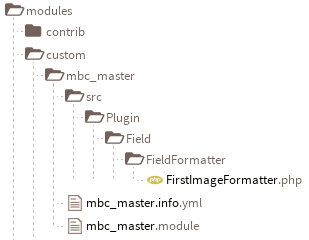
\includegraphics{mbc_master}

\subsection{Módulo 2 - MBC Review}
Este módulo foi criado com o objetivo de prover um método para o administrador do site enviar e-mail para usuários pedindo Reviews de produtos ou Opiniôes sobre a empresa, prover um link exclusivo para criação destes conteúdos que vai neste e-mail, que reconhece automaticamente o usuário e não publique este conteúdo, deixando-o para moderação do administrador.

\subsection{Módulo Adaptado - TinyPNG}
Por ser um módulo bem simples que utiliza uma biblioteca externa para fazer a minificação, a adptação deste módulo foi bem simples. Uma função que é executada quando uma entidade (conteúdo) é salva foi utilizada e usada a biblioteca tinify \url{packagist.org/packages/tinify/tinify} para executar a minificação das imagens. Além disso, o módulo adiciona uma página administrativa para ser gerenciada a chave da API do serviço, que pode ser obtida no site \url{https://tinypng.com/}.

\section{Resultado II}

TODO

TODO Schema.org

\chapter{Discussão}

\section{Melhorias}

\subsection{Minificação}
Mudar o serviço utilizado para minificação das imagens do site, ajudaria a melhorar a nota do site e sua performance, o que traria um benefício na indexação por motores de busca. As alternativas são OptiPNG e JpegOptim, ambas ferramentas de código livre. A dificuldade estaria em integrá-las com o Drupal, pois ambas são utilizadas em linha de comando.

\subsection{Funções Acicionais no E-commerce}
Para facilitar o rasteamento do pedido pelo usuário, fariamos uma área do cliente com todos os serviços relativos ao pedido como, por exemplo, rastreamento da encomenda, status do pagamento e histórico de pedidos.

\subsection{Calculadora de Frete}
Outro serviço interessante para se implementar, seria uma página de cálculo de frete, onde o usuário entra com informações como quantidade de balas e CEP em um formulário e tem como resposta as opções de frete e seus preços.

\subsection{Design}
A mudança mais necessária que vemos é um novo design. Por maior que seja o esforço feito, o design, que é um das principais características de um website, não ficou muito bom. Um trabalho de \textit{re-design} seria extramamente bem vindo e se possível feito por um profissional, que saiba como valorizar os principais pontos do site e o faça de maneira fluida e harmoniosa.

\chapter{Conclusão}

Pela falta de interesse momentâneo do cliente, o site não foi divulgado e sua função e-commerce está desabilitada. Por este motivo não pudemos resultados relevantes coletados de SEO, que necessita um site minimamente divulgado. Apesar disto, mesmo sem um conteúdo relevante, aparecer na primeira página em uma busca mostra que estamos no caminho certo e que quando colocar-mos o site 100\% online com um conteúdo bem produzido e com algumas campanhas de marketing, ele será muito melhor indexado.

A performance obtida foi altamente satisfatória, acima do esperado e atingindo o objetivo definido. A surpresa fica pelo tempo de resposta do servidor, que apesar de ser compartilhado e de baixo custo, mostrou-se bem rápido e capaz. A ferramenta GTMetrix ajudou na medição e também com dicas nos vários teste que foram realizados durante o desenvolvimento, sendo de suma importância para o projeto.

O e-commerce, apesar de não abilitado, funcionou muito bem nos testes e é esperado que quando colocado a disposição do publico, funcione sem problemas. Até o momento não foi testada uma compra real, com um número de cartão válido, somente compras com cartões de testes providos pelo PayPal, que em teoria seriam suficientes. As funções de envio de e-mail ao final da compra foram testadas e funcionam sem problemas. No geral, o e-commerce funciona como esperado, mas ainda sim, tem muito a melhorar.

Como dito no capitulo anterior, um ponto que não teve um resultado satisfatório foi o design. Apesar disto, vejo que a dificuldade de ter este ponto re-feito é mínima e o mais importante é que está funcional e bem programado.

Finalmente, o projeto como um todo, teve um resultado satisfatório na maioria do pontos dados como objetivos, superando as espectatívas em alguns. Foi um objeto bastante complexo, por ter passar por várias áreas de um sistema web, como servidor, back-end, front-end e SEO, e por isso, bastante valioso para o aprendizado.

% ----------------------------------------------------------
% ELEMENTOS PÓS-TEXTUAIS
% ----------------------------------------------------------
\postextual
% ----------------------------------------------------------

% ----------------------------------------------------------
% Referências bibliográficas
% ----------------------------------------------------------
\bibliographystyle{abbrv}
\bibliography{monografia}

% ----------------------------------------------------------
% Glossário
% ----------------------------------------------------------
%
% Consulte o manual da classe abntex2 para orientações sobre o glossário.
%
%\glossary

% ----------------------------------------------------------
% Apêndices
% ----------------------------------------------------------

% ---
% Inicia os apêndices
% ---
\begin{apendicesenv}

% Imprime uma página indicando o início dos apêndices
\partapendices
% ----------------------------------------------------------
\chapter{Quisque libero justo}
% ----------------------------------------------------------

\end{apendicesenv}
% ---

\end{document}
